% TEMPLATE for Usenix papers, specifically to meet requirements of
%  USENIX '05
% originally a template for producing IEEE-format articles using LaTeX.
%   written by Matthew Ward, CS Department, Worcester Polytechnic Institute.
% adapted by David Beazley for his excellent SWIG paper in Proceedings,
%   Tcl 96
% turned into a smartass generic template by De Clarke, with thanks to
%   both the above pioneers
% use at your own risk.  Complaints to /dev/null.
% make it two column with no page numbering, default is 10 point

% Munged by Fred Douglis <douglis@research.att.com> 10/97 to separate
% the .sty file from the LaTeX source template, so that people can
% more easily include the .sty file into an existing document.  Also
% changed to more closely follow the style guidelines as represented
% by the Word sample file. 

% Note that since 2010, USENIX does not require endnotes. If you want
% foot of page notes, don't include the endnotes package in the 
% usepackage command, below.

% This version uses the latex2e styles, not the very ancient 2.09 stuff.
\documentclass[letterpaper,twocolumn,10pt]{article}
\usepackage{usenix,epsfig,endnotes}
\begin{document}

%don't want date printed
\date{}

%make title bold and 14 pt font (Latex default is non-bold, 16 pt)
\title{\Large \bf Containerized Filesystems : A Performance Investigation of Containers across Filesystems}

%for single author (just remove % characters)
\author{
{\rm Jia R. Wu}\\
University of Waterloo
\and
{\rm Jichen Zhao}\\
University of Waterloo
% copy the following lines to add more authors
% \and
% {\rm Name}\\
%Name Institution
} % end author

\maketitle

% Use the following at camera-ready time to suppress page numbers.
% Comment it out when you first submit the paper for review.
\thispagestyle{empty}


\subsection*{Abstract}
Your Abstract Text Goes Here.  Just a few facts.
Whet our appetites.

Container as a Service (CaaS) platforms are being offered to personal and enterprise applications,  
In this paper, we attempt to profile the performance of three separate filesystems, ext4, reiserfs, and xfs running ontop of Arch Linux.



\section{Introduction}
Filesystems are the implementation of specific rules and principles governing how data is stored and retrieved on storage medium. At the time of writing, there are multiple various filesystems supported on the Linux operating system including ext4, reiserfs, xfs and many more. These filesystems all contain central concepts such as blocks and inodes, but differ subtly in their implementations (cite the linux documentation project here http://www.tldp.org/LDP/sag/html/filesystems.html).

Containers, also known as standardized units of software, are executables built ontop of a kernel. These containers offer a standardized execution environment agnostic to the environment the container is installed on. In this paper, we chose to examine Docker, a popular and free platform for creating and running containers. Docker has been championed by researchers as a platform which allows for reproducible research (cite https://arxiv.org/pdf/1410.0846.pdf).
We are interested in researching whether or not container based filesystem operations incur a significant performance overhead relative to native filesystem operations.


\section{Methods}

\subsection{Environment}
Jason Add Description of Your Computer Here

\subsection{Docker}


\subsection{Benchmarks}
Filebench, a popular filesystem and storage benchmark for I/O profiling is used to profile our three filesystems, as it permits custom and scalable workloads. We utilized five workloads which shipped with Filebench: FILESERVER, VARMAIL, VIDEOSERVER, WEBPROXY and WEBSERVER. Each of these benchmarks were called 5 times after a fresh installation of the filesystem. Temporary files were discarded with "rm -rf" after each benchmark prior to running the next benchmark to clear the cache. The runtime of Filebench benchmarks were fixed at 300 seconds with the exception of WEBPROXY. Unless explicitly mentioned, the benchmarks use the predefined settings given by the authors\endnote{The predefined settings can be located here: https://github.com/filebench/filebench/wiki/Predefined-personalities}. This was to mitigate any ramp-up effects that might occur with our HDD. We had to disable address space layout randomization by setting randomize\_va\_space=0 in /proc/sys/kernel so that Filebench would execute properly and give consistent results.

\subsubsection{FILESERVER}
This workload creates a directory tree, and calls a sequence of creates, deletes, appends, reads and writes on various files. The authors of Filebench describe this workload as being similar to SPECsfs. We configured the FILESERVER workload to output files of 1.2GB in size, with one flow for each stat, delete, read, close, append, open, close, write, and create operations.

\subsubsection{VARMAIL}
In this benchmark, multiple operations of create-append-sync, read-append-sync, read and delete are run in a single directory. The purpose of these operations are to simulate I/O operations on a mail server. 

\subsubsection{VIDEOSERVER}
This workload simulates a videoserver by serving video files from one directory and caching videos in a second directory. Videos were configured to be 3.2GB in size.

\subsubsection{WEBPROXY}
WEBPROXY simulated I/O on a web proxy server. Multiple files were created, written to, closed, and deleted in parallel. This benchmark was configured to run only for 60 seconds as 300 seconds would cause a segfault. The authors of Filebench are aware of this issue on Github.

\subsubsection{WEBSERVER}
This benchmark is similar to WEBPROXY, however it runs open-read-close operations on files in a directory tree and has an additional step of appending. 



\section{Results}


\begin{figure}[!h]
\centering
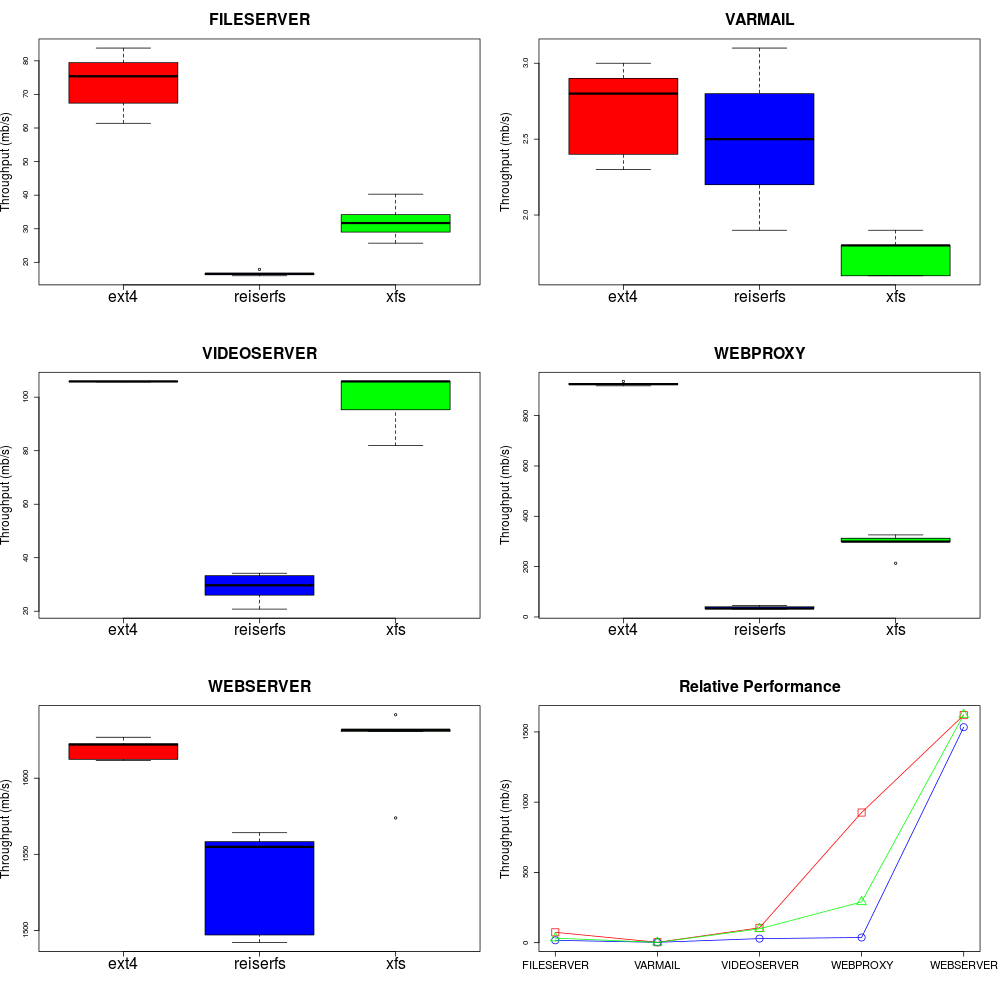
\includegraphics[width=3in]{../results/fs_benchmark_arch.png}
\caption{Native FileSystem Performance per Workload}
\label{fig:arch_workload_boxplots}
\end{figure}


\section{Discussion}
\subsection{Threats To Validity}
Well, it's getting boring isn't it.  This is the last subsection
before we wrap it up.

\section{Acknowledgments}

A polite author always includes acknowledgments.  Thank everyone,
especially those who funded the work. 

\section{Availability}
All relevant scripts and data can be retireved from the following repository:
\begin{center}
{\tt https://github.com/JRWu/fall2017\_cs854/\~{}myname/SWIG}
\end{center}


{\footnotesize \bibliographystyle{acm}
\bibliography{../common/bibliography}}


\theendnotes

\end{document}

